\documentclass[main.tex]{subfiles}

\begin{document}

\chapter{Learning Theory and Mathematical Methods}

Machine learning explores the study and construction of algorithms that are capable of finding patterns in data. Hence, this entails studying the ability of learning models to capture these patterns and generalize, as one would in statistical learning theory, in addition to studying model efficiency, enabled by computational complexity theory. In practice, many of the widely used supervised and unsupervised machine learning models can reasonably be described as linear algebraic data analysis techniques. For example, consider that ordinary least squares regression and ridge regression can be given in terms of a closed-form product of matrices and matrix inverses and that principal component analysis is essentially solving for the largest-eigenvalue eigenvectors of a particular covariance matrix. Furthermore, optimization problems, which are common in machine learning, can often be broken down into a set of basic linear algebraic subproblems.

\section{Classical Learning Theory}

We are given data from a training set $T$ and a test set $S$ of a subset $\Omega \subset \RR^d$. We assume that $S$ and $T$ are drawn from the same input space $X$. Furthermore, there exists output space $Y = \{ -1, +1 \} $ and a distribution $D$ on $X \times Y$.

Now, suppose we have a labelling $m: T \cup S \rightarrow Y$.  Our goal is to use this information to find some approximation function $\tilde{f} : X \rightarrow Y$ that minimizes estimation error for function class $F$. In other words, let true risk for function $f$ be defined as

\begin{align*}
R^{true}(f) = P_{X, Y \sim D}(f(X) \neq Y)	
\end{align*}

Then, estimation error is the difference in true risk between $\tilde{f}$ and optimal choice $f^* = \inf_{f \in F}R^{true}(f)$.

One classical method is using so-called Support Vector Machines (SVM), which construct a separating hyperplane such that the distance to the nearest training observation (minimum margin) is maximized. Much of the popularity of SVMs can be attributed to its association with the "kernel trick" which maps the data to a higher dimensional space so that it is separable or approximately separable.

Here, we suppose that the data is given classically and we seek to show that, in some cases, we can obtain a quantum advantage by either generating the separating hyperplane in quantum feature space or simply estimating the kernel function.

\section{Boolean Fourier Analysis}

\section{Randomized Linear Algebra}

\begin{definition} Total Variation Distance.
\label{def:tve}

Let $P$ and $Q$ be distinct probability measures on a $\sigma$-algebra $\mathcal{F}$ of subsets of the sample space $\Omega$. Then, the total variation distance is given by

\begin{align*}
\delta(P, Q) &= \sup_{A \in \mathcal{F}}\vert P(A) - Q(A)\vert
\end{align*}
\end{definition}

\begin{lemma}Hoeffding--Chernoff Inequality
\label{lem:chernoff}

Let $X_1, X_2, \cdots, X_s$	be i.i.d real random variables. For any positive, real numbers $a, t$ we have that, from Markov's inequality,

\begin{align*}
\Pr(\sum_{i=1}^s X_i \geq a) &\leq e^{-ta} E\Bigg[\prod_{i=1}^s e^{tX_i}\Bigg]\\
&= e^{-ta} \prod_{i=1}^s E\Bigg[e^{tX_i}\Bigg]
\end{align*}
by independence.
\qed
\end{lemma}

\begin{theorem}Hoeffding--Chernoff Inequality for matrix-valued random variables \cite{kannan2017randomized}
	
	Let $X$ be a random variable taking values which are real symmetric $d \times d$ matrices. Suppose $X_1, X_2, \cdots , X_s$ are i.i.d. draws of $X$. For any positive real numbers $a$, $t$, we have
	
	\begin{align}
		\label{thm:chern-mat-eigen}
		\Pr(\lambda_{\max}\Big(\sum_{i=1}^s X_i\Big) \geq a ) &\leq de^{-ta} \Vert E[e^{tX}]\Vert_2^s \\
		\label{thm:chern-mat-norm}
		\Pr(\Big\Vert \Big(\sum_{i=1}^s X_i\Big)\Big\Vert_2 \geq a ) &\leq de^{-ta} (\Vert E[e^{tX}]\Vert_2^s + \Vert E[e^{-tX}]\Vert_2^s)
	\end{align}
	
	where $\lambda_{\max}$ is the largest eigenvalue.
	\begin{proof}
		First, we can show that (\ref{thm:chern-mat-eigen}) $\implies$ (\ref{thm:chern-mat-norm}). By definition of the 2-norm of a matrix,
		
		\begin{align*}
		\Vert \sum_i X_i \Vert_2 = \max\Big(\lambda_{\max} \Big(\sum_i X_i\Big), \lambda_{\max} \Big(\sum_i (-X_i)\Big)\Big)	
		\end{align*}
		
		since it is the square root of the maximum eigenvalue of $(\sum_i X_i^T) \sum_i X_i = (\sum_i X_i) \sum_i X_i$ and hence, equivalently, the maximum absolute value of an eigenvalue of $X_i$. Therefore, we can simply apply (\ref{thm:chern-mat-eigen}) to both $X_i$ and $-X_i$ and we get (\ref{thm:chern-mat-norm}).
		
		So, we can focus our attention on (\ref{thm:chern-mat-norm}). Let $S = \sum_i^s X_i$. Hence,
		
		\begin{align*}
		\lambda_{\max}(S) \geq a \iff 	\lambda_{\max}(tS) \geq ta
		\intertext{Furthermore, by considering the power series definition of the exponential,}
		\iff \lambda_{\max}(e^{tS}) \geq e^{ta}\\
		\implies \Tr(e^{tS}) \geq e^{ta}
		\end{align*}
		
since the trace is the sum of the matrix's eigenvalues. Since $\Tr(e^{tS}) \geq 0$, we can apply Markov's inequality

\begin{align*}
\Pr(\Tr(e^{tS}) \geq e^{ta}) \leq \frac{E[\Tr(e^{tS})]}{e^{ta}}
\end{align*}

Now, we use the following lemma

\begin{lemma}
Golden-Thompson Inequality

If $A$ and $B$ are Hermitian matrices, then

\begin{align*}
\Tr(e^{A + B}) \leq \Tr(e^A e^B)
\end{align*}
\qed
\end{lemma}

Hence, we can let $A = t(\sum_i^{s-1} X_i)$ and $B = tX_s$. Then,

\begin{align*}
E_X\Big[\Tr(e^{tS})\Big] &\leq E_X\Big[\Tr(e^{t\big(\sum_i^{s-1} X_i\big)}e^{tX_s})\Big]\\
\shortintertext{Since the expectation operator commutes with the summation of the trace by linearity of trace,}
&= \Tr\Big(E_X\Big[e^{t\big(\sum_i^{s-1} X_i\big)}e^{tX_s}\Big]\Big)\\
&= \Tr\Big(E_{X_1, X_2, \cdots, X_{s-1}}\Big[e^{t\big(\sum_i^{s-1} X_i\big)}\Big]E_{X_s}\Big[e^{tX_s}\Big]\Big) \tag{by independence}\\
\end{align*}

Now, we can apply Corollary (\ref{cor:psd-tr-norm-ineq}), which gives 

\begin{align*}
&\leq \Tr\Big(E_{X_1, X_2, \cdots, X_{s-1}}\Big[e^{t\big(\sum_i^{s-1} X_i\big)}\Big]\Big) \Big\Vert E_{X_s}\Big[e^{tX_s}\Big]\Big\Vert_2\\
&= \Tr\Big(E_{X}\Big[e^{t\big(\sum_i^{s-1} X_i\big)}\Big]\Big) \Big\Vert E_{X}\Big[e^{tX}\Big]\Big\Vert_2 \\
&= E_X\Big[\Tr\Big(e^{t\big(\sum_i^{s-1} X_i\big)}\Big)\Big] \Big\Vert E_{X}\Big[e^{tX}\Big]\Big\Vert_2  \intertext{So we can repeat this process iteratively, peeling an $X_i$ each time from the left term. For clarity, the next step gives,}
E_X\Big[\Tr\Big(e^{t\big(\sum_i^{s-1} X_i\big)}\Big)\Big] &\leq E_X\Big[\Tr(e^{t\big(\sum_i^{s-2} X_i\big)}e^{tX_{s-1}})\Big]\\
&\leq E_X\Big[\Tr\Big(e^{t\big(\sum_i^{s-2} X_i\big)}\Big)\Big] \Big\Vert E_{X}\Big[e^{tX}\Big]\Big\Vert_2 \tag{applying (\ref{cor:psd-tr-norm-ineq}) again}
\intertext{Therefore, after peeling all terms but the last $X_i$, we have}
E_X\Big[\Tr(e^{tS})\Big] &\leq E_X\Big[\Tr\Big(e^{tX}\Big)\Big] \Big\Vert E_{X}\Big[e^{tX}\Big]\Big\Vert_2^{s-1} \intertext{Hence, since the trace is the sum of eigenvalues, $\Tr(e^{tX}) \leq d \lambda_{\max}(e^{tX})$ i.e. the worst case of all $d$ eigenvalues being the max}
&\leq d \Big\Vert E_{X}\Big[e^{tX}\Big]\Big\Vert_2^{s}
\end{align*}

as desired.
\end{proof}
\end{theorem}

\begin{lemma}
\label{lemma:exp-eigen-approx}
If $B \in \CC^{d \times d}$ is a hermitian matrix for which $\Vert B \Vert_2 \leq 1$, then $e^{B} \leq I + B + B^2$

\begin{proof}
	We know that $e^{\lambda_i} \leq 1 + \lambda_i + \lambda_i^2$, $|\lambda_i|^2 \leq 1$. Hence,
	
	\begin{align*}
	e^{\lambda_i} \ket{v_i}\bra{v_i} \leq (1 + \lambda_i + \lambda_i^2) 	\ket{v_i}\bra{v_i}
	\end{align*}

	where $\ket{v_i}$ is the corresponding eigenvector. This then implies
	
	\begin{align*}
	e^B &= \sum_{i=1}^d e^{\lambda_i} \ket{v_i}\bra{v_i} \preceq \sum_{i=1}^d (1 + \lambda_i + \lambda_i^2) \ket{v_i}\bra{v_i} \\
	&= I + B + B^2
	\end{align*}
\end{proof}
\end{lemma}

\chapter{A Review of Quantum Machine Learning}

\section{Introduction}

Since its conception, quantum computation and quantum information has taught us to "think physically about computation" \cite{nielsen2010quantum}. Well, if quantum mechanics tells us that physical states are mathematically linear algebraic objects (vectors in a Hilbert space), then perhaps this lesson says that the type of computation best suited for quantum physical reality are linear algebraic problems, such as the machine learning ones noted above. This somewhat naive intuition turns out to have value, as we will show in this review.

Hence, this leads us to the idea of quantum machine learning which uses quantum algorithms as part of a larger implementation to outperform the corresponding classical learning algorithms.

Nevertheless, past linear algebraic analysis techniques, there exist other classes of machine learning algorithms such as deep learning built on artificial neural networks and reinforcement learning which models an environment as a Markov decision process \cite{sutton1998reinforcement}. Successes have been achieved in terms of (potential) quantum speedups in these arenas \cite{dong2008quantum}, but we won't explore these alternative machine learning routes further in our review. 

In this chapter, we will cover the main theoretical results in terms of quantum algorithms relevant to quantum machine learning. Then, we'll describe specific learning problems that have achieved quantum speedups using these results. Finally, we'll discuss important limitations to these results which may pose substantive challenges to the future of quantum learning theory.

Our goal is to provide a birds-eye view of these concepts and refer the reader to appropriate references where they desire greater detail.

\section{Comparing Machine Learning Performance}

If we are to claim that some machine learning algorithms perform better on a quantum computer, we first must decide on a notion of "outperforming". 

This is currently characterized by the advantage in runtime obtained by a quantum algorithm over the classical methods for the same task. We quantify the runtime with the asymptotic scaling of the number of elementary operations used by the algorithm with respect to the size of the input, as one does in complexity theory. 

The definition of an elementary operation is dependent on the choice of measure of complexity. Query complexity measures the number of queries to the information source for the classical or quantum algorithm. Hence, a quantum speedup results if the number of queries needed to solve a problem is lower for the quantum than for the classical algorithm \cite{biamonte2017quantum}.

\section{Speedup Techniques}
   
\subsection{Solving Systems of Linear Equations}

Solving linear systems of equations is a ubiquitous problem in machine learning. As we will discuss, many learning problems, such as least-squares regression and least-squares SVMs, require the inversion of a matrix. Hence, we will describe two common quantum algorithms which lead up to the recent HHL algorithm, named after the algorithm's authors, Harrow, Hassidim, and LLoyd.

\subsubsection{HHL Algorithm}

One such application of Phase Estimation (Section \ref{phase_estimation}) is with respect to solving linear systems of equations. This is the so-called HHL algorithm \cite{lloyd2010quantum}. Here, we will cover the essential details of the algorithm.

The general problem statement of a linear system is if we are given matrix $A$ and unit vector $\vec{b}$, then find $\vec{x}$ satisfying, 

$$A\vec{x} = \vec{b}$$ 

However, assume that instead of solving for $x$ itself, we instead solve for an expectation value $x^T M x$ for some linear operator $M$. The original description of the algorithm provides runtime bound of $\tilde{O}(\log(N)\kappa ^{2} s^2 / \epsilon)$, where $s$ is sparsity measured by the maximum number of non-zero elements in a row and column of $A$, $\kappa$ is the condition number, and $\epsilon$ is the approximation precision. Hence, we can only achieve speedup if the linear system is sparse and has a low condition number $\kappa$. Ambainis \cite{ambainis2012variable} and Childs \cite{childs2015quantum} improved this depency on $\kappa$ and $s$ to linear and $\epsilon$ to poly-logarithmic.

This compares well considering that the best classical algorithm has a runtime of $O(N^{2.373})$ \cite{coppersmith1987matrix}. However, due to the large amount of pre-processing required, the algorithm is not used in practice. Standard methods, for example, based on QR-factorization take $O(N^3)$ steps \cite{golub2012matrix}. 

So, assume that $A$ in our linear system is an $N \times N$ Hermitian matrix. Notice that this is an "unrestrictive" constraint on $A$ because we can always take non-Hermitian matrix $A'$ and linear system $A' \vec{x} = \vec{b}$ and instead solve $\begin{bmatrix}
	0 && A' \\ A'^\dag && 0
\end{bmatrix} \begin{bmatrix} 0 \\ x \end{bmatrix} = \begin{bmatrix} b \\ 0 \end{bmatrix}$. Hence, we we will assume that $A$ is Hermitian from here on. 

Recall that because $A$ is hermitian, then we can perform quantum phase estimation using $e^{-iAt}$ as the unitary transformation. This can be done efficiently if $A$ is sparse.

So, we first prepare $\ket{b} = \sum_i b_i \ket{i}$ (the representation of $\vec{b}$). We assume that this can be done efficiently or that $\ket{b}$ is supplied as an input.

Denote by $\ket{\psi_j}$ the eigenvectors of $A$ with associated eigenvalues $\lambda_j$. Hence, we can express $\ket{b}$ as $\ket{b} = \sum_j \beta_j \ket{\psi_j}$.  So, we initialize a first register to state $\sum_j \beta_j \ket{\psi_j}$ and second register to state $\ket{0}$ . After applying phase estimation, we then have the joint state $\sum_j \beta_j \ket{\psi_j} \ket{\widetilde{\lambda}_j}$, where $\widetilde{\lambda}_j$ is an approximation of $\lambda_j$. We'll assume that this approximation is perfect from here on, for the sake of demonstration. 

Next we add an ancilla qubit and perform a rotation conditional on the first register which now holds $\ket{\lambda_j}$. The rotation transforms the system to

\begin{align*}
\sum_j \beta_j \ket{\psi_j} \ket{\lambda_j} \Big(\sqrt{1-\frac{C^2}{\lambda_j^2}}\ket{0} + \frac{C}{\lambda_j}\ket{1}\Big)
\end{align*}

for some small constant $C \in \RR$ that is $O(1/\kappa)$.

Hence, we can undo phase estimation to restore the second register to $\ket{0}$.

Now, if we measure the ancillary qubit in the computational basis, we'll evidently collapse the state to $\ket{1}$ with some probability. We'd then have

\begin{align*}
	\sum_j \frac{C}{\lambda_j} \beta_j \ket{\psi_j} \ket{\lambda_j}\ket{1} = C (A^{-1} \ket{b})
\end{align*}

In particular, the probability of getting this result is 

\begin{align*} 
	p(-1) &= \Bigg(\sum_j \beta_j \bra{\psi_j} \bra{\lambda_j} \Big(\sqrt{1-\frac{C^2}{\lambda_j^2}}\bra{0} + \frac{C}{\lambda_j}\bra{1}\Big) \Bigg)\ket{1}\bra{1} \Bigg(\sum_j \beta_j \ket{\psi_j} \ket{\lambda_j} \Big(\sqrt{1-\frac{C^2}{\lambda_j^2}}\ket{0} + \frac{C}{\lambda_j}\ket{1}\Big)\Bigg) \\
	&= \sum_j \beta_j \bra{\psi_j} \bra{\lambda_j} \Big(\sqrt{1-\frac{C^2}{\lambda_j^2}}\bra{0} + \frac{C}{\lambda_j}\bra{1}\Big) \ket{1}\bra{1} \beta_j \ket{\psi_j} \ket{\lambda_j} \Big(\sqrt{1-\frac{C^2}{\lambda_j^2}}\ket{0} + \frac{C}{\lambda_j}\ket{1}\Big) \\
	&= \sum_j \beta_j \bra{\psi_j} \bra{\lambda_j} \frac{C}{\lambda_j}\bra{1}\ket{1}\bra{1} \beta_j \ket{\psi_j} \ket{\lambda_j} \frac{C}{\lambda_j}\ket{1} \\
	&= \sum_j \beta_j^2 \frac{C^2}{\lambda_j^2} \\
	&= \| A^{-1} \ket{b} \|^2 C^2 = \Omega(1/\kappa^2)
\end{align*} 

However, using amplitude amplification (Section \ref{sec:search}) this can be upper-bounded to $O(1/\kappa)$. 

Finally, we can make a measurement $M$ whose expectation value $\bra{x}M\ket{x}$ corresponds to the feature of $x$ we wish to evaluate. 

The concessions we noted along the way clearly limit the algorithm's applicability to practical problems. We have three essential caveats to achieving exponential speedup: (1) $A$ must be sparse and have a condition number that scales at most sublinearly with $N$, (2) $\ket{b}$ must be loaded in quantum superposition in $\log(N)$ time, and (3) $\ket{x}$ isn't actually be read out, but instead an expectation is computed.

Limitation (1) has been partially resolved by the work of \cite{wossnig2018quantum} to achieve a quadratic speedup for dense matrices. 

Limitation (2) may be solved by quantum RAM, which then has its own limitations discussed in the next section. 

Limitation (3) is a general issue with regards to reading out classical information from a quantum state at the conclusion of a quantum algorithm because we would need at least $N$ measurements to retrieve this classical data. Hence, this would eliminate the potential for exponential speed-up.  

Hence, after observing these limitations we may wonder if there can exist a classical algorithm with the same caveats that can achieve the same runtime. Importantly, in the original paper the authors showed that HHL is “universal for quantum computation.” Hence, we can encode any quantum algorithm e.g. Shor's algorithm into a system of roughly $2^n$ linear equations in $2^n$ unknowns, and then use HHL to “solve” the system (i.e., simulate the algorithm) in polynomial time. Thus, provided we believe any quantum algorithm achieves an exponential speedup over the best possible classical algorithm, HHL can theoretically achieve such a speedup as well \cite{aaronson2015read}.

To conclude, HHL is a logarithmic time quantum algorithm for matrix inversion, a task arising in many learning problems. However, a number of caveats that include the requirement of a logarithmic access time to the memory and the impossibility of retrieving the solution vector with one measurement lead to the question of whether classical or parallel algorithms that make use of the same assumptions obtain similar, or better, runtimes in practice. Hence, we will need empirical data to further address this question.

\subsection{Quantum Random Access Memory} 

The essence of machine learning is analyzing a vast amount of data. Hence, we must address the question of how classical data is encoded in quantum superposition, a concern brought up in our previous discussion of the matrix inversion algorithm. 

So, assume that we have an classical vectors $\{v_1, \cdots , v_ n : v_1 \in \RR^m \}$ that need to be encoded for use as part of a quantum algorithm. Quantum random access memory (qRAM) can encode these classical vectors in superposition into $\log(nm)$ qubits in $\log(nm)$ time using its "bucket-brigade architecture"\cite{giovannetti2008quantum}. The basic idea is to use a three-level tree structure where the $nm$ qubit "leaves" contain the entries of the $n$ vectors in $\RR^m$.

One of the central limitations of qRAM is that the number of resources scales as $O(nm)$ i.e. exponentially in the binary representation of $n, m$. There have been open questions of the viability of this model of memory, in practice. In particular, if each of the qubits must be error-corrected, then it seems entirely impractical for general use. Some of this concern has been answered by proponents who have showed that, given a certain error model, algorithms that require to query the memory a polynomial number of times (e.g. the HLL algorithm above) might not require fault-tolerant components. Still, the amplitude amplification algorithm above does require this error correction. 

Furthermore, it may be only fair to compare qRAM to a parallel classical architecture, given that we are allowing resources to scale exponentially. 

Considerable, too, is the fact that data must be distribute fairly uniformly over the quantum register or else qRAM is no longer efficient \cite{aaronson2015read}. 

In conclusion, qRAM comes with a significant number of considerations in itself and hence should be subjected to empirical investigation to determine its genuine quantum speed-up in practice. 

%\section{Inner Product Evaluation}

\section{Applications}

\subsection{Principal Component Analysis}

First, we consider the ubiquitous principal component analysis (PCA) algorithm. PCA reduces the dimensionality of data by transforming the features to uncorrelated weightings of the original features ("principal components"). This requires simply finding the eigenvalues and eigenvectors of the data covariance matrix. 

Hence, let $v_j \in V$ where $V$ is a $d$-dimensional vector space such that $d=2^n=N$ and assume that $|v_j| = 1$ for simplicity. Hence, the covariance matrix of the data is given by $C = \sum_j v_jv_j^T$ whose eigenvalues and eigenvectors we seek to discover. So, suppose we can prepare quantum state $v_j \rightarrow \ket{v_j}$, choosing classical data vector $v_j$ uniformly at random. For example, we can use qRAM, discussed above. Then, because of our random selection, the resulting quantum state has density matrix $\rho = \frac{1}{N} \sum_j \ket{v_j}\bra{v_j}$ which we observe to be the covariance matrix, up to an overall factor. 

Then, as Lloyd, Mohseni and Rebentrost describe \cite{lloyd2014quantum}, one way to perform quantum PCA use that given $n$ copies of $\rho$ we have the ability to apply the unitary operator $e^{-i\rho t}$ to any state $\sigma$ with accuracy $O(t^2 / n)$. This can be done by using repeated infinitesmal applications of the SWAP operator on $\rho \otimes \sigma$. 

Hence, using $e^{-i \rho t}$, we can perform phase estimation on $rho$. So, let $\ket{\psi_i}$ be the eigenvectors of $\rho$ with associated eigenvalues $\lambda_i$ and so $\rho = \sum_j \lambda_j \ket{\psi_j}\bra{\psi_j}$. Therefore, phase estimation gives u

\begin{align*}
\sum_j \lambda_j \ket{\psi_j}\bra{\psi_j} \otimes \ket{\tilde{\lambda_j}} \bra{\tilde{\lambda_j}}
\end{align*}

where $\tilde{\lambda_j}$ is an approximation of $\lambda_j$. Hence, if we measure the second register and repeat this procedure several times, the most frequent outcome is the first principal component $\ket{\psi_{max}}$, and so on.

The algorithm works best when a small number of principal components have significantly greater eigenvalues than the rest. Hence, $\rho$ is well represented by the subspace spanned by the principal components. In particular, let $m << d$ be the dimension of the subspace of principal components which represent $\rho$ within some bound. Then, the algorithm has runtime $O(m \log n )$. 

Hence, this gives a limitation: if the eigenvalues of the covariance are roughly equal and of size $O(1/d)$, then the algorithm reduces to scaling in time $O(d)$ (as does the classical algorithm). Furthermore, we evidently inherit the limitations of qRAM, if we use it for the state preparation above.  

\subsection{Support Vector Machines}

Support vector machines seek to find an optimal (maximum margin) separating hyperplane between two classes of data in a dataset. Hence, if the training data is linearly separable, each class can be found on only one side of the hyperplane. In particular, let $\{ x_1 , \cdots , x_n \}$ be a set of observations where $x_i$ is a $d$-dimensional vector with associated labels $y_i \in \{ 0 , 1\}$. Hence, we seek a linear function $f(x) = \vec{w} \cdot \vec{x} - \vec{b}$ where $\vec{w}$ is a weight vector and $\vec{b}$ is a bias vector s.t. $y_if(x_i) > 0, \forall i$. Furthermore, we seek to maximize the minimum $y_i f(x_i)$, across all $i$. 

\begin{figure}[H]
\centering
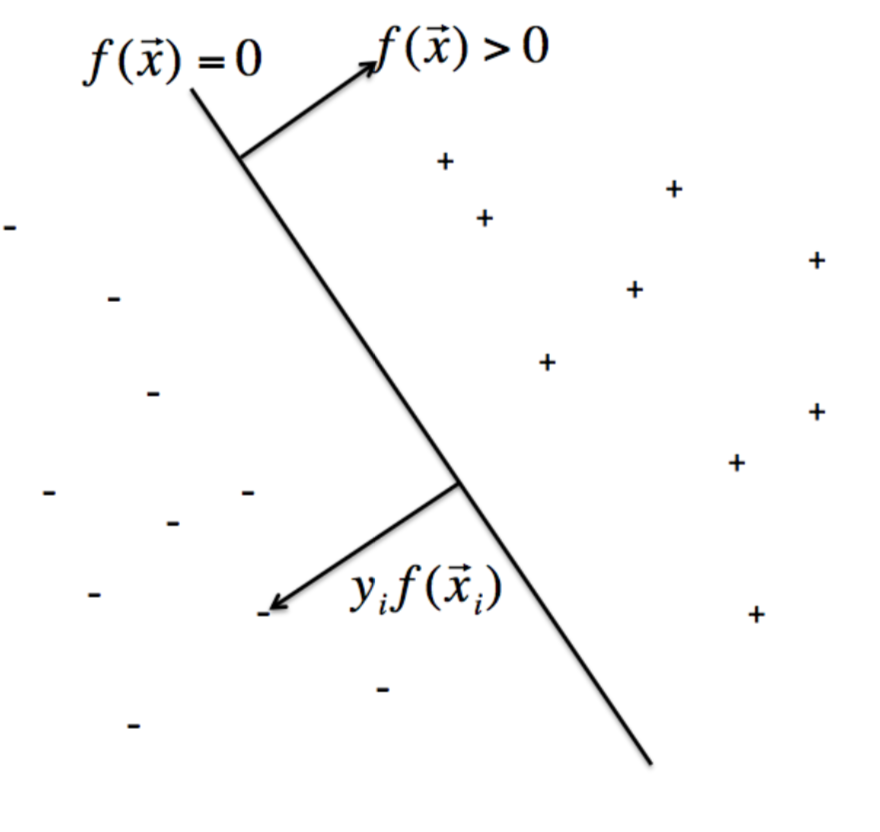
\includegraphics[width=0.5\linewidth]{images/svm.png}	
\caption{Visualization of a separating hyperplane and its associated margin taken from \cite{rudin}.}
\end{figure}

Much of the appeal of SVM is in its generalization to nonlinear hypersurfaces by replacing the constituent inner products with a kernel that implicitly maps the observations to another high dimensional space \cite{rudin}.% This mapping can be represented by a kernel ma

Solving SVM generally is performed by optimization of the dual problem which is a quadratic optimization problem. Hence, in \cite{rebentrost2014quantum}, the authors show that quantum evaluation of inner products leads to exponential speed-ups in terms of $d$. 

Full exponential improvements, however, can be achieved (with respect to $d$ and $n$) in the case of least-squares SVMs \cite{rebentrost2014quantum}. In this case, finding a solution requires optimizing a least squares minimization. Hence, this type of minimization reduces to solving a set of linear equations. So, after data has been inputted efficiently (perhaps using qRAM), a modified version of the matrix inversion algorithm above can be used, incorporating methods from the PCA algorithm above to prepare the linear system.

The key point is, all the operations required to construct the maximum-margin separating hyperplane and to test whether a vector's classification can be performed in time that is polynomial in $\log n$.

%\subsection{Generative Adversarial Networks}

\subsection{Gaussian Processes}

In \cite{zhao2018quantum}, the authors demonstrate an application of HHL algorithm with respect to Gaussian process regression (GPR), another supervised learning method. In effect, GPR is a stochastic generalization of ordinary regression. In particular, let $\{ x_1 , \cdots , x_n \}$ be a set of observations where $x_i$ is a $d$-dimensional vector with associated scalar targets $y_i$. In GPR, we consider the distribution over latent functions $f(x)$ which can return the correct labelling, $y$, given an inputted data-point. However, we further assume that this labelling is subject to Gaussian noise i.e. $f(x) = y + \epsilon$, where $\epsilon$ is the Gaussian noise. Hence, GPR uses Bayesian inference to return this distribution of latent functions such that they are consistent with the observed data. 

Now, given this distribution and some test input $x'$, we can predict its output by computing (1) a linear predictor known as the predictive mean and (2) the variance of the predictor with respect to $x'$. These values then give the distribution the $y'$ that is consistent with training data. Hence, the quantum speedup comes from the fact that both of these values can be computed using a modification of the HHL algorithm, as described in \cite{zhao2018quantum}. Furthermore, the size of the output is independent from the size of the dataset which the authors use to show that, combined with the efficiency of HHL, can given exponential speedups in terms of $d$. Again, we require that the data can be loaded in efficiently initially e.g. using qRAM.  

\subsection{Optimization}

Unsurprisingly, optimization methods are fundamental to many machine learning algorithms. Again, we can apply our quantum set of tools to several important optimization problems, including semi-definite programs (with potential super-polynomial speedups) and constraint satisfiability programs. Even easier to see, we can directly use our demonstrated results to solve quadratic programming problems which reduce to a linear system. If $N \times N$ matrices that define the linear system are sparse and low rank, we can use HHL and yield a solution in $\log N$ time--an exponential speedup.

Furthermore, iterative optimization, such as by means of gradient descent can be implemented by modifying PCA. In this case, several copies of a quantum state representing the solution are used to iteratively improve the solution. We may expect improvements in this type of optimization to lead to improvement in training neural networks on a quantum computer. 

Interestingly, the quantum optimization algorithm finds approximate solutions for combinatorial optimization by "alternating qubit rotations with the application of the problem's penalty function" \cite{biamonte2017quantum}.

\subsection{Topological Data Analysis}

By now, we've seen that the presented algorithms suffer from a common limitation: the classical data must be loaded into a quantum superposition efficiently given that the speedups come from performing the computational steps after data is loaded in. However, this issue can be avoided in cases where the data points can be computed efficiently individually, as opposed to loading all of a large dataset in. In terms of machine learning, this can happen when the computation component of the algorithm requires exploring a comparatively small subset of the original dataset. In other words, if we can explore a subset of the input data to determine the distribution and other descriptive features of the overall data, we can then have the quantum algorithm generate the combinatorially larger space in quantum parallel, thereby computing the quantum dataset efficiently. This idea was used in the context of topological data analysis in \cite{lloyd2016quantum}.

Topological features, in particular, seem promising for this goal given that they are independent of the metric of choice and hence capture essential features of the data. In a discrete set, topological features are given by features that persist across spatial resolutions. These persistent features, formalized through persistent homology, are less likely to be artifacts of noise or parameterization. For example, the holes, voids, or connected components are examples of such features. The number of these types of features are defined for simplical complex (roughly a closed set of simplexes) as "Betti numbers". 

In the paper, the authors show how to generate quantum states to encode the simplexes using logarithmically fewer qubits. Furthermore, they show that the Betti numbers can be efficiently represented using this representation. Important assumptions were made, in particular such that the quantum state encoding the simplexes can be generated efficiently. One satisfying condition is if the number of simplexes in the complex are exponentially large. Hence, in at least some cases, we may extract exponential speed-ups in this type of topological analysis.

\section{Challenges}

The first obvious challenge to quantum machine learning is that the execution of quantum algorithms requires quantum hardware that does not exist at present. 

Aside from this, as we've seen by now, many of the quantum algorithms which are used to potentially give quantum speedups come with several caveats and limitations to their use. As noted in \cite{biamonte2017quantum}, implicitly in \cite{aaronson2015read}, and repeatedly elsewhere, we can condense the general caveats into a few fundamental problems: 

(1) The Input State Preparation Problem. The cost of reading in the input can in some cases dominate the cost of quantum algorithms. In many cases, we hoped qRAM would solve this problem. Understanding this factor is an important ongoing challenge.

(2) The Readout problem. Retrieving the solution in terms of classical information after performing quantum algorithms requires learning an exponential number of bits through repeated trials. We've shown that learning an expectation value of a linear operator can be a sound alternative (e.g. in the case of matrix inversion).

(3) The true cost problem. We require empirical study to show the number of gates or elementary operations to carry out a quantum algorithm, in practice. For example, we encountered this issue in the fundamental phase estimation algorithm (i.e. is it fair to assume that a $U^{2^j}$ gate is an elementary operation?). Nevertheless, our query complexity bounds seem to indicate great advantages in specific cases, as we've noted.

Throughout this review, we've considered learning classical data which introduces problems (1) and (2), given that we have to interface between classical and quantum states. Hence, we may consider the case of applying quantum algorithms to quantum data. This is covered in detail in \cite{aaronson2007learnability}.

\section{Supervised learning with quantum feature Hilbert spaces}
\cite{havlicek2018supervised}


\subsection{Feature Map}

Consider the feature vector kernel $K(x, z) = | \bra{\Phi(x)}\ket{\Phi(z)} |^2$

\subsection{Quantum Variational Classification}

\subsection{Quantum Kernel Estimation}

\subsection{Non-Trivial Feature Map with Entanglement}

\subsection{Geometric Analysis of Candidate Feature Maps}

\subsection{Experimental Simulation of Candidate Feature Maps}

%\section{Density Matrix Exponentiation Algorithms}
%\url{https://www.nature.com/articles/nphys3029}
%
%\section{Review of Quantum Machine Learning}
%\url{https://www.nature.com/articles/nature23474}
%
%\section{Learnability of Quantum States}
%\begin{enumerate}
%\item \url{https://arxiv.org/abs/quant-ph/0608142}
%\item \url{https://arxiv.org/abs/1711.01053}
%\item \url{https://arxiv.org/abs/1801.05721}
%\end{enumerate}


\section{Quantum-Inspired Length-Square Sampling}

As we've seen, most well-known QML algorithms convert input quantum states to a desired output state or value. Thus, they do not provide a routine to get necessary copies of these input states (a state preparation routine) and a strategy to extract information from an output state. Both are essential to making the algorithm useful.

We've also seen that that many of the initial "practical" quantum algorithms attempted to workaround this difficulty by considering low-rank linear algebraic problems (poly-logarithmic in matrix dimension). For example, the data fitting algorithm \cite{wiebe2012quantum} allows one to compute $A^+ \ket{b} = \ket{x_{LS}}$ in $\tilde{O}(log(N)(s^3\kappa^6)/ \epsilon)$ time (query complexity) by using the HHL algorithm and matrix multiplication. Hence, we require that $A$ is sparse with low condition number $\kappa$ as well.

Nevertheless, these low-rank quantum algorithms still have substantial help from an assumed input state preparation routine which has been shown to be at least $\Omega(\sqrt{n})$ in vector input size (\cite{tang2018quantum}). Hence, a natural question to ask is whether there's a similar classical data structure which takes time polynomial in quantum state preparation which can offer machine learning algorithms with similar guarantees. In particular, we compare quantum algorithms with quantum state preparation to classical algorithms with sample and query access to input.	

\subsubsection{Definitions}

\begin{definition}
We have "query access" to $x \in \CC^n$ if, given $i \in [n]$, we can efficiently compute $x_i$. We say that $x \in \mathcal{Q}$.
\end{definition}
\begin{definition} We have sample \textbf{and} query access to $x \in \CC^n$ if 

\begin{enumerate}
\item We have query access to $x$ i.e. $x\in \mathcal{Q}$ ($\implies$ $\mathcal{SQ} \subset \mathcal{Q}$)
\item can produce independent random samples $i \in [n]$ where we sample $i$ with probability $|x_i|^2/\|x\|^2∣$ and can query for $\|x\|$.
\end{enumerate}
We say that $x \in \mathcal{SQ}$. 
\end{definition}
\begin{definition} For $A \in \CC^{m\times n}$, $A \in \mathcal{SQ}$ (abuse) if

\begin{enumerate}
\item $A_i \in \mathcal{SQ}$ where $A_i$ is the $i$th row of $A$
\item $\tilde{A} \in \mathcal{SQ}$ for $\tilde{A}$ the vector of row norms (so $\tilde{A}_i = \|A_i\|$).	
\end{enumerate}
\end{definition}


\begin{example}
Say we have the vector $\vec{x} = (2, 0, 1, 3)$ and $\vec{x} \in \mathcal{SQ}$. Consider the following binary tree data structure.
\end{example}

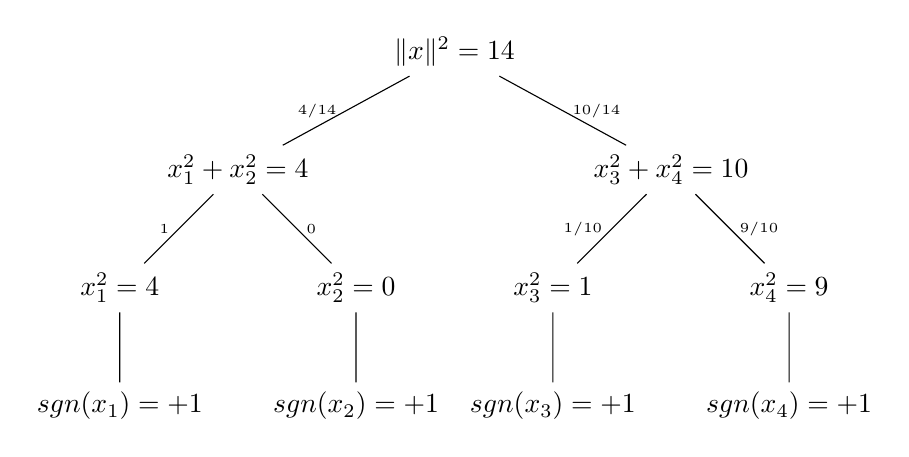
\begin{tikzpicture}[level distance=1.5cm,
  level 1/.style={sibling distance=5.5cm},
  level 2/.style={sibling distance=3cm}, 
  level 3/.style={sibling distance=3cm}]
  \node (1){$\| x \|^2 = 14$}
    child {node {$x_1^2 + x_2^2 = 4$}
      child {node {$x_1^2 = 4$}
      	child {node {$\text{sgn}(x_1) = +1$}}
      	edge from parent node [left] {\tiny $1$}
      }
      child {node {$x_2^2 = 0$} 
      	child {node {$\text{sgn}(x_2) = +1$}}
      	edge from parent node [right] {\tiny $0$}
      }
      edge from parent node [left] {\tiny $4/14$}
    }
    child {node(2) {$x_3^2 + x_4^2 = 10$}
    	child {node {$x_3^2 = 1$}
    		child {node {$\text{sgn}(x_3) = +1$}}
    		edge from parent node [left] {\tiny $1/10$}
    	}
      child {node(3) {$x_4^2 = 9$} 
      		child {node {$\text{sgn}(x_4) = +1$}}
      		edge from parent node [right] {\tiny $9/10$}
      } 
      edge from parent node [right] {\tiny $10/14$}
    };
\end{tikzpicture}



\subsubsection{Low-Rank Estimation}

The first tool we can construct given these sampling assumptions is a classical analog to quantum phase estimation (Section \ref{phase_estimation}).

\begin{itemize}
\item For $A \in \CC^{m\times n}$, given $A \in \mathcal{SQ}$ and some threshold $k$, we can output a description of a low-rank approximation of $A$ with $\text{poly}(k)$ queries.
\item Specifically, we output two matrices $S,\hat{U}\in \mathcal{SQ}$ where $S \in \CC^{\ell \times n}$, $\hat{U} \in \CC^{\ell \times k}$ ($\ell = \text{poly}(k,\frac{1}{\epsilon}$)), and this implicitly describes the low-rank approximation to $A$, $D := A(S^\dagger\hat{U})(S^\dagger\hat{U})^\dag$ ($\implies$ rank $D \leq k$).

\item This matrix satisfies the following low-rank guarantee with probability $\geq 1-\delta$: for $\sigma := \sqrt{2/k}\|A\|_F$, and $A_{\sigma} := \sum_{\sigma_i \geq \sigma} \sigma_iu_iv_i^\dag$ (using SVD), 
$$\|A - D\|_F^2 \leq \|A - A_\sigma\|_F^2 + \epsilon^2\|A\|_F^2$$
\item Note the $\|A - A_\sigma\|_F^2$ term. This says that our guarantee is weak if $A$ has no large singular values. 
\item Quantum analog: phase estimation
\end{itemize}


$$
\begin{bmatrix}
\\
\cdots A \cdots 
\\
\\	
\end{bmatrix}
\begin{bmatrix}
\\
S^\dag
\\
\\	
\end{bmatrix}
\begin{bmatrix}
\hat{U}
\end{bmatrix}
\begin{bmatrix}
\hat{U^\dag}
\end{bmatrix}
\begin{bmatrix}
\cdots S \cdots
\end{bmatrix}
$$

\subsubsection{Trace Inner Product Estimation}

\begin{itemize}
	\item For $x, y \in \CC^n$, if we are given that $x \in \mathcal{SQ}$ and $y \in \mathcal{Q}$, then we can estimate $\< x, y\>$ with probability $\geq 1 - \delta$ and error $\epsilon \|x\|\|y\|$ 
	\item Quantum analog: SWAP test
\end{itemize}

\begin{figure}
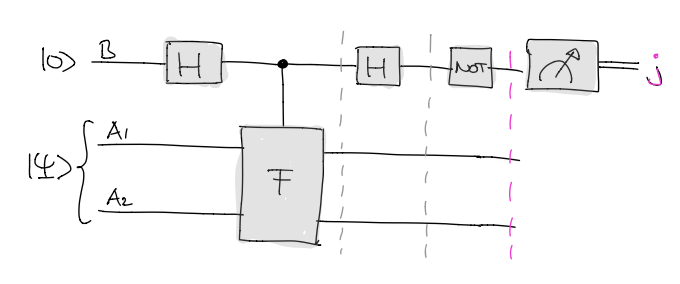
\includegraphics[width= 0.5\linewidth]{images/swap_test.png}	
\caption{Swap test}
\end{figure}

\begin{fact} For $\{X_{i,j}\}$ i.i.d random variables with mean $\mu$ and variance $\sigma^2$, let 

$$Y := \underset{j \in [\log 1/\delta]}{\operatorname{median}}\;\underset{i \in [1/\epsilon^2]}{\operatorname{mean}}\;X_{i,j}$$

Then $\vert Y - \mu\vert \leq \epsilon\sigma$ with probability $\geq 1-\delta$, using only $O(\frac{1}{\epsilon^2}\log\frac{1}{\delta})$ samples.
\end{fact}

\begin{itemize}
	\item In words: We may create a mean estimator from $1/\epsilon^2$ samples of $X$. We compute the median of $\log 1/\delta$ such estimators
	\item Catoni (2012) shows that Chebyshev's inequality is the best guarantee one can provide when considering pure empirical mean estimators for an unknown distribution (and finite $\mu, \sigma$)
	\item "Median of means" provides an exponential improvement in probability of success ($1 - \delta$) guarantee
\end{itemize}

\begin{corollary} For $x,y \in\CC^n$, given $x \in \mathcal{SQ}$ and $y \in \mathcal{Q}$, we can estimate $\langle x,y\rangle$ to $\epsilon\|x\|\|y\|$ error with probability $\geq 1-\delta$ with query complexity $O(\frac{1}{\epsilon^2}\log\frac{1}{\delta})$
\end{corollary}
\begin{proof}Sample an \textbf{index} $s$ from $x$. Then, define $Z := x_s y_s\frac{\|y\|^2}{|y_s|^2}$. Apply the Fact with $X_{i,j}$ being independent samples $Z$.
\end{proof}	

\subsubsection{Least-Square Sample Generation}

\begin{itemize}
	\item For $V \in \CC^{n\times k}, w \in \CC^k$, given $V^\dagger \in \mathcal{SQ}$ (\textit{column}-wise sampling of $V$) and $w \in \mathcal{Q}$, we can simulate $Vw \in \mathcal{SQ}$ with $\text{poly}(k)$ queries
	\item In words: if we can least-square sample the columns of matrix $V$ and query the entries of vector $w$, then
\begin{enumerate}
\item  We can query entries of their multiplication ($Vw$) 
\item We can least-square sample from a distribution that emulates their multiplication	
\end{enumerate}

\item Hence, as long as $k \ll n$, we can perform  each using a number of steps polynomial in the number of columns of $V$. 

\end{itemize}

\begin{definition}
Rejection sampling
\end{definition}
\begin{algorithm}
Input: Samples from distribution $P$

Output: Samples from distribution $Q$
\begin{itemize}
\item Sample $s$ from $P$
\item Compute $r_s = \frac{1}{N}\frac{Q(s)}{P(s)}$, for fixed constant $N$
\item Output $s$ with probability $r_s$ and restart otherwise
\end{itemize}
\end{algorithm}

\begin{fact}
Fact. If $r_i \leq 1, \forall i$, then the above procedure is well-defined and outputs a sample from $Q$ in $N$ iterations in expectation.	
\end{fact}


\begin{proposition}
	 For $V \in \RR^{n\times k}$ and $w \in \RR^k$, given $V^\dag \in \mathcal{SQ}$ and $w \in \mathcal{Q}$, we can simulate $Vw \in \mathcal{SQ}$ with expected query complexity $\tilde{O}((\frac{1}{\epsilon^2}\log\frac{1}{\delta}))$

We can compute entries $(Vw)_i$ with $O(k)$ queries.

We can sample using rejection sampling:

\begin{itemize}
\item $P$ is the distribution formed by sampling from $V_{(\cdot, j)}$.
  
\item $Q$ is the target $Vw$.
\item Hence, compute $r_s$ to be a constant factor of $Q / P$
\end{itemize}

$$r_i = \frac{\|w^T V_{\cdot, i}\|^2}{\|w\|^2\|V_{\cdot, i}\|^2}$$
\end{proposition}

\begin{itemize}
\item Notice that we can compute these $r_i$'s (in fact, despite that we cannot compute probabilities from the target distribution), and that the rejection sampling guarantee is satisfied (via Cauchy-Schwarz).

\item Since the probability of success is $\|Vw\|^2/ \| w\|^2$, it suffices to estimate the probability of success of this rejection sampling process to estimate this norm.

\item Through a Chernoff bound, we see that the average of $O(\|w\|^2(\frac{1}{\epsilon^2}\log\frac{1}{\delta}))$ "coin flips" is in $[(1-\epsilon)\|Vw\|,(1+\epsilon)\|Vw\|]$ with probability $\geq 1-\delta$.
\end{itemize}

\subsubsection{Application: Stochastic Regression}

For a low-rank matrix $A \in \RR^{m\times n}$
  and a vector $b \in \RR^n$, given $b, A \in \mathcal{SQ}$, (approximately) simulate $A^+b \in \mathcal{SQ}$.

\begin{algorithm}   	
\begin{itemize}
\item Low-rank approximation (3) gives us $S,\hat{U} \in \mathcal{SQ}$.

\item Applying thin-matrix vector (2), we get $\hat{V} \in \mathcal{SQ}$, where $\hat{V} := S^T\hat{U}$; we can show that the columns of $\hat{V}$ behave like the right singular vectors of $A$.
\item Let $\hat{U}$ have columns $\{ \hat{u}_i\}$. Hence, $\hat{V}$ has columns $\{ S \hat{u}_i \}$. Write its $i$th column as $\hat{v}_i := S\hat{u}_i$.

\item Low-rank approximation (3) also outputs the approximate singular values $\hat{\sigma}_i$ of $A$
\end{itemize}
\end{algorithm}

Now, we can write the approximate vector we wish to sample in terms of these approximations:

$$A^+b = (A^TA)^+A^Tb \approx \sum_{i=1}^k \frac{1}{\hat{\sigma}_i^2}\hat{v}_i\hat{v}_i^T A^Tb$$

\begin{itemize}
\item We approximate $\hat{v}_i^TA^Tb$ to additive error for all by noticing that $\hat{v}_i^TA^Tb = \tr(A^Tb\hat{v}_i^T)$ is an inner product of $A^T$ and $b\hat{v}_i^T$. 
\item Thus, we can apply (1), since being given $A \in \mathcal{SQ}$ implies $A^T \in \mathcal{SQ}$ for $A^T$ viewed as a long vector. 
\item Define the approximation of $\hat{v}_i^TA^Tb$ to be $\hat{\lambda}_i$. At this point we have (recalling that $\hat{v}_i := S\hat{u}_i$)

$$A^+b \approx \sum_{i=1}^k \frac{1}{\hat{\sigma}_i^2}\hat{v}_i\hat{\lambda}_i = S \sum_{i=1}^k \frac{1}{\hat{\sigma}_i^2}\hat{u}_i\hat{\lambda}_i$$

\item Finally, using (2) to provide sample access to each $S \hat{u}_i$, we are done	! $\tilde{O}(\kappa^{16}k^6 \|A\|^6_F / \epsilon^6)$ complexity.
\end{itemize}


\subsubsection{Definitions and Assumptions}

Let $b \in \CC^m$ and $A \in \CC^{m \times n}$ s.t. $\Vert A \Vert \leq 1$ where $\Vert \cdot \Vert$ signifies the operator norm (or spectral norm). Furthermore, require that $\rank(A) = k$ and $\Vert A^+ \Vert \leq \kappa$ where $A^+$ is the pseudoinverse of $A$. Hence, observe that $\Vert A \Vert \leq 1$ is equivalent to $A$ having maximum singular value $1$\footnote{To see this, simply consider Spectral Theorem applied to Hermitian matrix $A^\dag A$}. Similarly, $A^+$ has inverted singular values from $A$ and so $\Vert A^+ \Vert$ is equal to the reciprocal of the minimum nonzero singular value. Therefore, the condition number of $A$ is given by $\Vert A \Vert \Vert A^+ \Vert \leq \kappa$.

So, define $x$ to be the least-squares solution to the linear system $Ax = b$ i.e. $x = A^+ b$. Then, in terms of these definitions, we define two primary goals:

\begin{enumerate}
\item Query a vector $\tilde{x}$ s.t. $\Vert \tilde{x} - x \Vert \leq \epsilon \Vert x \Vert$
\item Sample from a distribution that approximates $\frac{|x_j|^2}{\Vert x \Vert^2}$ within total variation distance (\autoref{def:tve}) $2\epsilon$.
\end{enumerate}

In order to do this, we simply assume that we have length-square sampling access to $A$. In other words, we are able to sample row indices of $A$ from the distribution $\frac{\Vert A_{(i, \cdot)}\Vert^2}{\Vert A \Vert^2_F}$

\subsubsection{Sequence of Approximations}

First, we'll summarize the sequence of approximations that we'll perform using length-squared sampling techniques. We'll describe these steps in depth in the following sections.

Of course, we know that the least squares solution of the linear system is given by the orthogonal projection

\begin{align*}
	(A^\dag A)^+ A^\dag = A^+ b
\end{align*}

So, we first approximate $A^\dag A$ by $R^\dag R$ where $R \in \CC^{r \times n}$, $r \ll m$ is constructed from length-square sampling $r$ rows of $A$. Now, denote the spectral decomposition 

\begin{align*}
A^\dag A \approx R^\dag R = \sum_{l=1}^k \frac{1}{\sigma_l^2}\ket{v^{(l)}}\bra{v^{(l)}}
\end{align*}

where of course $\sigma_i$ and $\ket{v^{(i)}} \in \CC^n$ are the singular values and right singular vectors of $R$, respectively.

We see that computing these right singular vectors of $R$ can still be computationally prohibitive given the dimension $n$. Hence, we can use length-square sampling again, this time on the columns of $R$ to give a matrix $C \in \CC^{r \times c}$, $c \ll n$. Now, the left singular vectors of $C$ which we denote as $\ket{w^{(i)}} \in \CC^r$ can be efficiently computed via standard SVD methods. So,

\begin{align*}
RR^\dag \approx CC^\dag = \sum_{l=1}^k \frac{1}{\sigma_l^2}\ket{w^{(l)}}\bra{w^{(l)}}
\end{align*}


We can then show that ()

\begin{align}
\label{def:approx-right}
\ket{\tilde{v}^{(i)}} := R^\dag \ket{w^{(l)}} / \tilde{\sigma}_l
\end{align}

provides a good approximation of $\ket{v^{(i)}}$. Note that $\tilde{\sigma}_l$ are the singular values of $C$ which then approximate the singular values of $R$ which similarly approximate the singular values of $A$. This follows from $A^\dag A \approx R^\dag R$ and $RR^\dag \approx CC^\dag$ by the Hoffman--Wielandt inequality detailed in Lemma 2.7 of \cite{kannan2017randomized} and stated without proof below.

\begin{lemma}Hoffman--Wielandt inequality

	If $P, Q$ are two real, symmetric $n \times n$ matrices and $\lambda_1, \cdots \lambda_n$ denote eigenvalues in non-decreasing order, then
	
	\begin{align*}
		\sum_{t=1}^n(\lambda_t(P) - \lambda_t(Q))^2 \leq \Vert P - Q \Vert_F^2
	\end{align*}
\end{lemma}


At this point, it seems like we haven't made much progress since computing $R^\dag \ket{w^{(l)}}$ is still expensive. However, it turns out that all we need to enable query access to $\tilde{x}$ is the ability to efficiently estimate the trace inner product $\tr(U^\dag V)$ where $U$ and $V$ are operators such that $U$ can be the length-square sampled and $V$ can be queried. To see this, we write our solution, $\tilde{x}$, in terms of the approximations thus far

\begin{align*}
	\tilde{x} &\approx A^+ \ket{b} \\
	&\approx (R^\dag R)^+ A^\dag \ket{b}\\
	&\approx \sum_{l = 1}^k \frac{1}{\tilde{\sigma}_l^2} \ket{\tilde{v}^{(l)}} \bra{\tilde{v}^{(l)}} A^\dag \ket{b}
\end{align*}

Hence, define $U := A$, $V := \ket{b}\bra{\tilde{v}^{(l)}}$ in which case 

\begin{align*}
\tr(U^\dag V) &= \tr(A^\dag \ket{b} \bra{\tilde{v}^{(l)}}) \\
&= \tr(\bra{\tilde{v}^{(l)}} A^\dag \ket{b} )\\
&= \bra{\tilde{v}^{(l)}} A^\dag \ket{b}
\end{align*}

since $\bra{\tilde{v}^{(l)}} A^\dag \ket{b}$ is a scalar. Therefore, say that 

$$
\tilde{\lambda}_l \approx \tr(A^\dag \ket{b} \bra{\tilde{v}^{(l)}})
$$

and assume that we can compute and memoize these scalars $\tilde{\lambda}_i$ efficiently. In which case,

\begin{align*}
\tilde{x} &\approx \sum_{l = 1}^k \frac{1}{\tilde{\sigma}_l^2} \ket{\tilde{v}^{(l)}} \tilde{\lambda}_l
\intertext{Recalling the definition of $\ket{\tilde{v}^{(i)}}$ (\ref{def:approx-right}),}
&= \sum_{l = 1}^k \frac{1}{\tilde{\sigma}_l^3} R^\dag \ket{w^{(l)}} \tilde{\lambda}_l\\
&= R^\dag \sum_{l = 1}^k \frac{1}{\tilde{\sigma}_l^3} \ket{w^{(l)}} \tilde{\lambda}_l
\intertext{and so defining $z := \sum_{l = 1}^k \frac{1}{\tilde{\sigma}_l^3} \ket{w^{(l)}} \tilde{\lambda}_l$,}
&= R^\dag z
\end{align*}

We see that we can compute $z$ efficiently (and memoize it for future queries) because it is a $k$-linear combination of left singular vectors in $\CC^r$. So, say that we wish to query an element $\tilde{x}_j$. We can simply query column $R_{\cdot, j} \in \CC^r$ (or equivalently row $R_{j, \cdot}^\dag$) and compute $R_{\cdot, j} \cdot z$. Hence, we've achieved our first goal.

In order to achieve our second goal, enabling sample access to a distribution that approximates $\frac{|x_j|^2}{\Vert x \Vert^2}$, we require one more trick: rejection sampling which we detail in Section ().

All in all, we've performed the chain of approximations,

\begin{align*}
	\ket{x} &= A^+ \ket{b} = (A^\dag A)^+ A^\dag \ket{b}\\
	&\approx (R^\dag R)^+ A^\dag \ket{b} = \sum_{l = 1}^k \frac{1}{\tilde{\sigma}_l^2} \ket{v^{(l)}} \bra{v^{(l)}} A^\dag \ket{b}\\
	&\approx \sum_{l = 1}^k \frac{1}{\tilde{\sigma}_l^2} \ket{\tilde{v}^{(l)}} \bra{\tilde{v}^{(l)}} A^\dag \ket{b}\\ %\qquad \Big(\ket{\tilde{v}^{(l)}} := R^\dag \ket{w^{(l)}}\Big)
	&\approx \sum_{l = 1}^k \frac{1}{\tilde{\sigma}_l^2} \ket{\tilde{v}^{(l)}} \tilde{\lambda}_l = R^\dag \sum_{l = 1}^k \frac{1}{\tilde{\sigma}_l^3} \ket{w^{(l)}} \tilde{\lambda}_l = R^\dag z
\end{align*}


Now that we've sketched the steps of this process, we detail each approximation and show that we can achieve the claimed correctness and complexity bounds.

\subsubsection{Computing Approximate Singular Vectors}

As described above, we begin by length-square sampling the original matrix $A \in \CC^{m \times n }$. Suppose we want to draw $s$ rows in $s$ i.i.d. trials. Then, pick row index $i$ of $A$ with probability

\begin{align}
\label{def:A-prob}
p_i = \frac{\Vert A_{(i, \cdot)}\Vert^2}{\Vert A \Vert_F^2} 	
\end{align}

and output random row 

\begin{align*}
 	Y &= \frac{1}{\sqrt{s p_i}} \bra{A_{(i, \cdot)}} \\\
 	&= \frac{1}{\sqrt{s}}\frac{\Vert A\Vert_F}{\Vert A_{(i, \cdot)}\Vert}\bra{A_{(i, \cdot)}}
\end{align*}

which is just a scaling of the $i$th row of $A$\footnote{The reason that we scale by $s$ is so that the expectations of $A^\dag A$ and $R^\dag R$ coincide in the theorem that follows. The reason that we scale by $p_i$ is so that the norms of all rows are equivalent---a fact which we'll utilize when we sample $R$ column-wise.}. In other words,

\begin{align*}
\Pr(Y = \frac{1}{\sqrt{s p_i}} \bra{A_{(i, \cdot)}}) = p_i
\end{align*}


After sampling $s$ rows, we implicitly define matrix $R$ to be the concatenation of the outputted random rows. Therefore,

\begin{align}
\label{def:R}
R &= \begin{bmatrix}
Y_1 \\
Y_2 \\
\vdots \\
Y_s
\end{bmatrix} \in \CC^{s \times n}
\end{align}

Note that $\bra{Y_k}$ denotes the random row outputted by the procedure on the $k$th i.i.d. draw.

\begin{lemma}
	Let $X = Y^\dag Y - E[Y^\dag Y]$ which evidently satisfies $E[X] = 0$. Then,
	
	\begin{align}
	E[X^2] &\preceq E[(Y^\dag Y)^2] \\
	&= A^\dag A \Vert A \Vert_F^2 \frac{1}{s^2}	
	\end{align}
	
	and so 
	
	\begin{align}
	\label{eq:expect-x-2}
	\Vert E[X^2] \Vert_2 \leq \frac{1}{s^2} \Vert A \Vert_2^2 \Vert A \Vert_F^2	
	\end{align}

	
	Furthermore,
	
	\begin{align}
	\Vert X \Vert_2 = \frac{1}{s} \Vert A \Vert^2_F	
	\end{align}
\begin{proof}
First, observe that $E[X^2]$ is the element-wise variance of $Y^\dag Y$ and $E[(Y^\dag Y)^2]$ is the corresponding second moment. Hence, the relation $E[X^2] \leq E[(Y^\dag Y)^2]$ holds element-wise which implies that the matrix relation $E[X^2] \preceq E[(Y^\dag Y)^2]$ holds as well.

Furthermore, 

\begin{align*}
E[(Y^\dag Y)^2] &= \frac{1}{s^2} \sum_{i = 1}^m \frac{p_{i}}{p_{i}^2} \ket{A_{(i, \cdot)}}\bra{A_{(i, \cdot)}}\ket{A_{(i, \cdot)}}\bra{A_{(i, \cdot)}} \\
&= \frac{1}{s^2} \sum_{i = 1}^m \frac{\Vert A \Vert_F^2}{\bra{A_{(i, \cdot)}}\ket{A_{(i, \cdot)}}} \ket{A_{(i, \cdot)}}\bra{A_{(i, \cdot)}}\ket{A_{(i, \cdot)}}\bra{A_{(i, \cdot)}}\tag{using (\ref{def:A-prob})}\\
&= \frac{1}{s^2} \sum_{i = 1}^m \Vert A \Vert_F^2 \ket{A_{(i, \cdot)}}\bra{A_{(i, \cdot)}} = \frac{\Vert A \Vert_F^2}{s^2} \sum_{i = 1}^m  \ket{A_{(i, \cdot)}}\bra{A_{(i, \cdot)}} \\
&= A^\dag A \Vert A \Vert_F^2 \frac{1}{s^2}	
\end{align*}

Recall that $E[R^\dag R] = \frac{1}{s} A^\dag A$. So, observe that

\begin{align*}
\Vert X \Vert_2 &= \Vert Y^\dag Y - E[Y^\dag Y] \Vert_2 \\
&= \frac{1}{s}\Bigg\Vert\frac{1}{p_i}\ket{A_{(i, \cdot)}}\bra{A_{(i, \cdot)}} - A^\dag A \Bigg\Vert_2 \\
&\leq \frac{1}{s} \max\Big\{ \Big\Vert\frac{1}{p_i}\ket{A_{(i, \cdot)}}\bra{A_{(i, \cdot)}}\Big\Vert_2 ,  \Big\Vert A^\dag A \Big\Vert_2\Big\}\\
&\leq \frac{1}{s} \max\Big\{ \frac{\Vert A \Vert_F^2}{\Vert \ket{A_{(i, \cdot)}} \Vert_2^2}\Big \Vert \ket{A_{(i, \cdot)}}\bra{A_{(i, \cdot)}}\Big\Vert_2 ,  \Vert A^\dag A \Vert_F^2\Big\} \intertext{using $\Vert A^\dag A \Vert_2 = \Vert A \Vert_2^2 \leq \Vert A \Vert_F^2$ and plugging in (\ref{def:A-prob}).}\\
&= \frac{1}{s} \Vert A \Vert^2_F	
\end{align*}
\end{proof}
\end{lemma}


\begin{proposition}
\label{prop:expect-exp-mat-norm}
	If $t > 0, t \in \CC$ satisfies $\Vert tX \Vert_2 \leq 1$ for all possible values of $X$, then 
	
	\begin{align}
	\begin{split}
	\Vert E[e^{\pm tX}] \Vert_2 &\leq 1 + \frac{t^2}{s^2} \Vert A \Vert_2^2 \Vert A \Vert_F^2 \\
	&\leq e^{t^2 \Vert A\Vert_2^2 \Vert A \Vert_F^2 / s^2}	
	\end{split}
	\end{align}
	
	\begin{proof}
		First, from (\ref{lemma:exp-eigen-approx}) we know that $E[e^{tX}] \preceq E[I + X + X^2] = I + E[X^2]$ since $E[X] = 0$. Hence, we have the proposition by (\ref{eq:expect-x-2}).
	\end{proof}
\end{proposition}

\begin{theorem}
Let $A \in \CC^{m \times n}$ and $R \in \CC^{r \times n}$ be constructed by the length-square sampling and scaling so that $E[R^\dag R] = E[A^\dag A]$ (requirements that are met by $R$ defined in (\ref{def:R})). Then, for all $\epsilon \in [0, \Vert A \Vert / \Vert A \Vert_F]$\footnote{If $\epsilon \geq \Vert A \Vert / \Vert A \Vert_F$, then we can simply use $\hat{0}$ to approximate $A^\dag A$}, we have

\begin{align*}
\Pr(\Vert R^\dag R - A^\dag A \Vert \geq \Vert A \Vert \Vert A \Vert_F) \leq 2ne^{\frac{- \epsilon^2 s}{4}}	
\end{align*}

Hence, for $s \geq (4 \ln \frac{2n}{\eta}) / \epsilon^2$, with probability at least $(1 - \eta)$ we have

\begin{align*}
	\Vert R^\dag R - A^\dag A \Vert \leq \epsilon\Vert A \Vert \Vert A \Vert_F
\end{align*}

\begin{proof}
	From our definition above, we have that 
	
	\begin{align*}
		R^\dag R &= \begin{bmatrix}
Y_1^\dag &
Y_2^\dag &
\hdots &
Y_s^\dag
\end{bmatrix}\begin{bmatrix}
Y_1 \\
Y_2 \\
\vdots \\
Y_s
\end{bmatrix} \\
&= \sum_{k=1}^s \ket{Y_k}\bra{Y_k} \intertext{Let $i_k$ give the index of the row sampled from $A$ on the $k$th draw. Hence, }\\
&= \frac{1}{s} \sum_{k=1}^s \frac{1}{p_{i_k}} \ket{A_{(i_k, \cdot)}}\bra{A_{(i_k, \cdot)}}
\end{align*}

Furthermore,

\begin{align*}
E[R^\dag R] &= 	\frac{1}{s} \sum_{k=1}^s \sum_{i_k = 1}^m \frac{p_{i_k}}{p_{i_k}} \ket{A_{(i_k, \cdot)}}\bra{A_{(i_k, \cdot)}} \\
&= \frac{1}{s} \sum_{k=1}^s A^\dag A \\
&= A^\dag A
\end{align*}

Note that similarly $E[Y^\dag Y] = \frac{1}{s} A^\dag A$.

So, we can define $X_i = \ket{Y_k}\bra{Y_k} - E\Big[\ket{Y_k}\bra{Y_k}\Big]$ which is evidently an i.i.d. copy of $X$ as we've defined previously. Hence,

\begin{align*}
\sum_{i=1}^s X_i &= R^\dag R - E[R^\dag R] \\
&= R^\dag R - A^\dag A	
\end{align*}

Now, we can first apply Theorem \ref{thm:chern-mat-eigen} with $a = \epsilon \Vert A \Vert_2 \Vert A \Vert_F$,

\begin{align*}
\Pr(\Big\Vert \Big(\sum_{i=1}^s X_i\Big)\Big\Vert_2 \geq \epsilon \Vert A \Vert_2 \Vert A \Vert_F ) \\ &\leq ne^{-t \epsilon \Vert A \Vert_2 \Vert A \Vert_F} (\Vert E[e^{tX}]\Vert_2^s + \Vert E[e^{-tX}]\Vert_2^s)	
\intertext{for any $t > 0$. Hence, we can apply Proposition \ref{prop:expect-exp-mat-norm} which then gives us}\\
	&\leq 2ne^{-t \epsilon \Vert A \Vert_2 \Vert A \Vert_F} e^{t^2 \Vert A\Vert_2^2 \Vert A \Vert_F^2 / s^2}	
	\intertext{for $t \leq s / \Vert A \Vert_F^2$. Hence, we can set $t = \frac{\epsilon s}{2 \Vert A \Vert_F \Vert A \Vert_2}$ (which is indeed less than $s / \Vert A \Vert_F^2$) and finally,}
	&\leq 2ne^{- \epsilon^2 s / 4}
\end{align*}

Therefore, if we require that $s \geq (4 \ln \frac{2n}{\eta}) / \epsilon^2$ we then have

\begin{align*}
\Pr(\Big\Vert \Big(\sum_{i=1}^s X_i\Big)\Big\Vert_2 \geq \epsilon \Vert A \Vert_2 \Vert A \Vert_F ) &\leq 2ne^{- \frac{\epsilon^2}{4} \frac{4 \ln \frac{2n}{\eta}}{ \epsilon^2}} \\
&= 2ne^{- \ln \frac{2n}{\eta}} = \eta
\end{align*}
\end{proof}
\end{theorem}


\subsection{Conclusions}

\begin{itemize}
\item Claim (Tang): For machine learning problems, $\mathcal{SQ}$ assumptions are more reasonable than state preparation assumptions.
\item We discussed pseudo-inverse which inverts singular values, but in principle we could have applied any function to the singular values
\item Gilyen et. al (2018) show that many quantum machine learning algorithms indeed apply polynomial functions to singular values
\item Our discussion suggests that exponential quantum speedups are tightly related to problems where high-rank matrices play a crucial role (e.g. Hamiltonian simulation or QFT)
\end{itemize}

\section{Optimal Quantum Sample Complexity}

It is well known that one can tightly bound the number of samples from an unknown distribution required to "probably approximately correctly" (PAC) learn an unknown concept in terms of its VC dimension (Section \ref{}). Hence, a natural question to ask is whether "quantum samples" are more powerful in the sense of requiring less examples to achieve this goal.

Here we will explore the techniques of Arunachalam and de Wolf \cite{arunachalam2016optimal} in order to address this question. The authors show that the ideas of quantum state discrimination discussed in Section \ref{} offer an intuitive analysis, despite resulting in a suboptimal lower bound. However, Boolean Fourier analysis (Section \ref{}) applied to the Pretty Good Measurement (Section \ref{}) gives an optimal bound showing that there is no quantum advantage in terms of sample complexity when restricting to PAC learning and quantum samples as specified in the model introduced by Bshouty and Jackson \cite{bshouty1998learning}.

\subsection{Definitions}

\subsubsection{Quantum Learning Models: PAC Setting}

A quantum example oracle $QPEX(c,D)$ acts on $\ket{0}^{\otimes n}\ket{0}$ and produces a quantum example $\sum_{x\in\{0,1\}^n} D(x)\ket{x,c(x)}$.

A quantum learner is given access to some copies of the state generated by $QPEX(c,D)$ and performs a POVM where each outcome is associated with a hypothesis. 

A learning algorithm $A$ is an $(\epsilon, \delta)$-PAC quantum learner for $C$ if for every $c \in C$ and distribution $D$, given access to the $QPEX(c,D)$ oracle, $A$ outputs an $h$ such that $err_D (h, c) \leq \epsilon$, with probability at least $1 - \delta$.

The sample complexity of $A$ is the maximum number invocations of the $QPEX(c,D)$ oracle, maximized over all $c \in C$ , distributions $D$, and the learner’s internal randomness. The $(\epsilon, \delta)$-PAC quantum sample complexity of a concept class $C$ is the minimum sample complexity over all $(\epsilon,\delta)$-PAC quantum learners for $C$.

\subsubsection{Quantum Learning Models: Agnostic Setting}

For a joint distribution $D : \{0, 1\}^{n+1} \rightarrow [0, 1]$ over the set of examples, the learner has access to an $QAEX(D)$ oracle which acts on $\ket{0}^{\otimes n}\ket{0}$ and produces a quantum example $\sum_{(x, b)\in\{0,1\}^{n+1}} D(x,b)\ket{x,b}$. 

A learning algorithm A is an $(\epsilon, \delta)$-agnostic quantum learner for $C$ if for every distribution $D$, given access to the $QAEX(D)$ oracle, $A$ outputs an $h \in C$ such that $err_D (h) \leq opt_D(h) + \epsilon$ with probability at least $1 - \delta$.

The sample complexity of $A$ is the maximum number invocations of the $QAEX(D)$ oracle over all distributions $D$ and over the learner’s internal randomness. The $(\epsilon, \delta)$-agnostic quantum sample complexity of a concept class $C$ is the minimum sample complexity over all $(\epsilon, \delta)$-agnostic quantum learners for $C$.

\subsection{Goals}

We seek to show that quantum examples are not actually more powerful than classical labeled examples in the PAC model and in the agnostic model when the underlying data distribution is arbitrary. We emphasize this point on the data distribution because we plan to later detail advantages that can be reaped if the example distribution is e.g. uniform (hint: think about the Bernstein-Vazirani algorithm and perceptron).

In the classical case, the sample complexity of concept class $\mathcal{C}$ with VC dimension $d$ in the PAC setting is

$$
\Theta(\frac{d}{\epsilon} + \frac{\log(1/\delta)}{\epsilon})
$$

where $\epsilon$ is the approximation coefficient and $\delta$ is the probability of success, as usual.

In the agnostic case, the optimal sample complexity of such agnostic learners is tightly determined by the VC dimension of $\mathcal{C}$

\begin{align*}
\Theta(\frac{d}{\epsilon^2} + \frac{\log(1/\delta)}{\epsilon^2})
\end{align*}

The authors indeed show that, using the quantum learning models above, the bounds are the same in the quantum case. This requires a state identification argument which uses Fourier Analysis to analyze the performance of a Pretty Good Measurement\ref{app:pgm}. However, we can get close by instead using simple concepts from quantum information theory. In my view, this approach has a strong aesthetic and is likely transferrable to similar problems.

Of course, we know that the upper bounds in sample complexity are the same as the classical case since we can always implement a classical algorithm on a quantum computer. Hence, we seek lower bounds instead. 

\subsection{Information Theoretic Lower Bounds on Sample Complexity}

\subsubsection{VC-independent lower bounds}

\begin{lemma}
Let $\mathcal{C}$ be a non-trivial concept class. For every $\delta \in (0,1/2), \epsilon \in (0,1/4)$, a $(\epsilon,\delta)$-PAC quantum learner for $\mathcal{C}$ has sample complexity $\Omega(\frac{1}{\epsilon}\log \frac{1}{\delta})$
\end{lemma}

\begin{proof} 
Since $\mathcal{C}$ is non-trivial, we may assume there are two concepts $c_1,c_2 \in C$ defined on two inputs $\{x_1,x_2\}$ as follows $c_1(x_1) = c_2(x_1) = 0$ and $c_1(x_2) = 0,c_2(x_2) = 1$.

 Consider the distribution $D(x_1) = 1−\epsilon$ and $D(x_2) = \epsilon$. For $i \in \{1,2\}$, the state of the algorithm after $T$ queries to $QPEX(c_i,D)$ is
 
 $$
 \ket{\psi_i} = (\sqrt{1-\epsilon}\ket{x_1, 0} + \sqrt{\epsilon}\ket{x_2, c_i(x_2)})^{\otimes T}
 $$
 
 Therefore, $\bra{\psi_1}\ket{\psi_2} = (1-\epsilon)^T$. Since the success probability of an $(\epsilon, \delta)$-PAC quantum learner is $\geq 1 - \delta$, Corollary \ref{cor:distinguish-two-pure-states} implies $\ket{\psi_1}\ket{\psi_2} \leq 2\sqrt{\delta(1-\delta)}$. 
 
 $\therefore T = \Omega(\frac{1}{\epsilon}\log \frac{1}{\delta})$
\end{proof}

\begin{lemma}
Let $\mathcal{C}$ be a non-trivial concept class. For every $\delta \in (0,1/2), \epsilon \in (0,1/4)$, a $(\epsilon,\delta)$-agnostic quantum learner for $\mathcal{C}$ has sample complexity $\Omega(\frac{1}{\epsilon^2}\log \frac{1}{\delta})$
\end{lemma}

\begin{proof}
Since $\mathcal{C}$ is non-trivial, we may assume there are two concepts $c_1,c_2 \in C$ defined on two inputs $\{x_1,x_2\}$ such that $c_1(x) \neq c_2(x)$.

 Consider the two distributions $D_\pm$ s.t.
 
 \begin{align*}
 	D_\pm(x, c_1(x)) &= (1 \pm \epsilon)/2\\
 	D_\pm(x, c_2(x)) &= (1 \mp \epsilon)/2\\
 \end{align*}
 $D_+(x_1) = 1−\epsilon$ and $D(x_2) = \epsilon$. The state of the algorithm after $T$ queries to $QAEX(D_\pm)$ is
 
 $$
 \ket{\psi_\pm} = ((\sqrt{(1\pm\epsilon)/2})\ket{x, c_1(x)} + (\sqrt{(1\mp\epsilon)/2})\ket{x, c_2(x)})^{\otimes T}
 $$
 
 Therefore, $\bra{\psi_+}\ket{\psi_-} = (1-\epsilon^2)^{T/2}$. Since the success probability of an $(\epsilon, \delta)$-agnostic quantum learner is $\geq 1 - \delta$, Corollary \ref{cor:distinguish-two-pure-states} implies $\bra{\psi_+}\ket{\psi_-} \leq 2\sqrt{\delta(1-\delta)}$. 
 
 $\therefore T = \Omega(\frac{1}{\epsilon^2}\log \frac{1}{\delta})$
\end{proof}


\subsubsection{Classical PAC Learning}

\begin{theorem}
Let $C$ be a concept class with $VC-dim(\mathcal{C}) = d + 1$. Then for every $\delta \in (0,1/2)$ and $\epsilon \in (0,1/4)$, every $(\epsilon,\delta)$-PAC learner for $\mathcal{C}$ has sample complexity $\Omega(\frac{d}{\epsilon} + \frac{\log(1/\delta)}{\epsilon})$.
\end{theorem}

\begin{proof} 
Consider an $(\epsilon,\delta)$-PAC learner for $\mathcal{C}$ that uses $T$ examples. The $d$-independent part of the lower bound, T = Ω(log(1/δ)/ε), even holds for quantum examples and was proven in Lemma 10. 

Hence it remains to prove T = Ω(d/ε). It suffices to show this for a specific distribution D, defined as follows. Let S = {s0,s1,...,sd} ⊆ {0,1}n be some (d + 1)-element set shattered by C . Define D(s0) = 1−4ε and D(si) = 4ε/d for all i ∈ [d].
Because S is shattered by C , for each string a ∈ {0, 1}d , there exists a concept ca ∈ C such that ca(s0) = 0 and ca(si) = ai for all i ∈ [d]. We define two correlated random variables A and B corresponding to the concept and to the examples, respectively. Let A be a random variable that is uniformly distributed over {0, 1}d ; if A = a, let B = B1 . . . BT be T i.i.d. examples from ca according to D. We give the following three-step analysis of these random variables:
1. I(A:B)≥(1−δ)(1−H(1/4))d−H(δ)=Ω(d).
Proof. Let random variable h(B) ∈ {0, 1}d be the hypothesis that the learner produces (given
the examples in B) restricted to the elements s1,...,sd. Note that the error of the hypothesis
\end{proof}

\section{Online Learning of Quantum States}

\subsection{Goals}

We will prove that

\begin{theorem}
	Let $E_1, E_2, \cdots$ be a sequence of two-outcome measurements on an $n$-qubit state presented to the learner, and $l_1, l_2, \cdots$ be the corresponding loss functions revealed in successive iterations in the regret minimization model. Suppose $l_t$ is convex and $L$-lipschitz; in particular for every $x \in \RR$, there is a subderivative $l_t'(x)$ such that $| l_t'(x)| \leq L$. Then there is an explicit learning strategy that guarantees regret $R_T = O(L \sqrt{Tn})$ for all $T$. This is so even assuming the measurement $E_t$ and loss function $l_t$ are chosen adaptively, in response to the learner's previous behavior. 
	
	Specifically, the algorithm applies to $L_1$ loss and $L_2$ loss, and achieves regret $O(\sqrt{Tn})$ for both. 
\end{theorem}


\subsection{Online Learning and Regret}


\end{document}